\section{Additional results for other tissue types and effective constitutive model forms} \label{sec:otherresults}

	Bovine pericardium is a good soft tissue to start with due high axes stretch coupling from their broad fiber splays. However, soft tissue behavior is drastically different with greater degree and anisotropy. For example aortic valve leaflets have larger elastin content resulting in larger toe region and extremely narrow ODFs, which can cause contraction along the material axis under equi-biaxial tension \cite{billiar_biaxial_2000b}. This behavior is hard for most constitutive models to replicate. However, $\Psi_{eff}$ (Eqn. \ref{eqn:finalexponentialmodelformscaled}) has no problem replicating this behavior (Fig. \ref{fig:aorticfit}). 

%%%%%%%%%%%%%%%%%%%%%%%%%%%%%%%%%%%%%%%%%%%%%%%%%%%%%%%%%%%%
%-------------------	begin FIGURE 	-------------------%
\begin{figure}
\centering
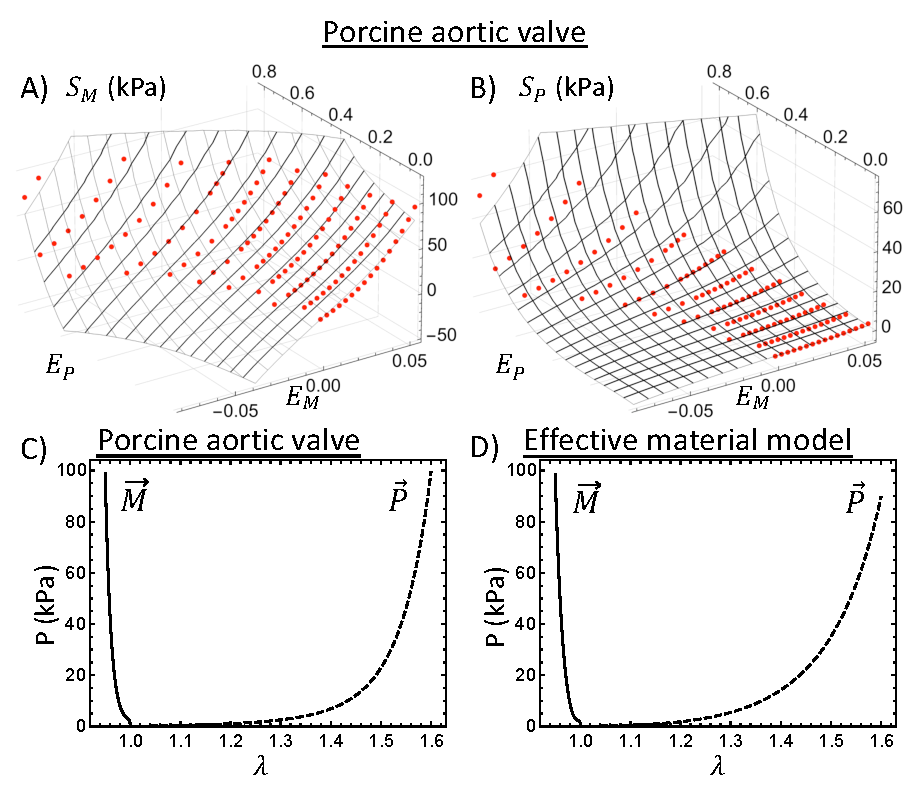
\includegraphics[width=6.5in]{Figures/aorticfit}
\caption{Parameter estimation results for porcine aortic valve specimen with highly align collagen fibers, $\sigma_{ODF} =10\deg$. The response function A) $S_m$ and b) $S_n$ are shown. C) This specimen contracts in the preferred fiber direction under equi-biaxial tension, a trait of soft tissues with highly aligned collagen fibers. D) $\Psi_{eff}$ (Eqn. \ref{eqn:finalexponentialmodelformscaled}) is able to reproduce this effect.}
\label{fig:aorticfit}
\end{figure} 
%-------------------	 end FIGURE 	-------------------%
%%%%%%%%%%%%%%%%%%%%%%%%%%%%%%%%%%%%%%%%%%%%%%%%%%%%%%%%%%%%
    
    Based on D-optimality, we determined the optimal loading paths and shown its importance for model predictability. The equi-biaxial stress loading path (near equi-biaxial) came out as especially important, as it is included in all sets of optimal loading paths except for two and four (Fig. \ref{fig:oddpaths}\&\ref{fig:evenpaths}). Commonly, when reproducing results from older publication, only the equi-biaxial stress loading path may be included in the figures as it is the most informative. Indeed, using the equi-biaxial stress loading paths simply results in much higher D-optimality than other choices. However, using this loading path alone is not sufficient for parameter estimation. Although the quality of fit is very good (Fig. \ref{fig:effequifit}A\&B), it cannot predict other loading paths (Fig. \ref{fig:effequifit}C\&D) 
    
%%%%%%%%%%%%%%%%%%%%%%%%%%%%%%%%%%%%%%%%%%%%%%%%%%%%%%%%%%%%
%-------------------	begin FIGURE 	-------------------%
\begin{figure}[!hbtp]
\centering
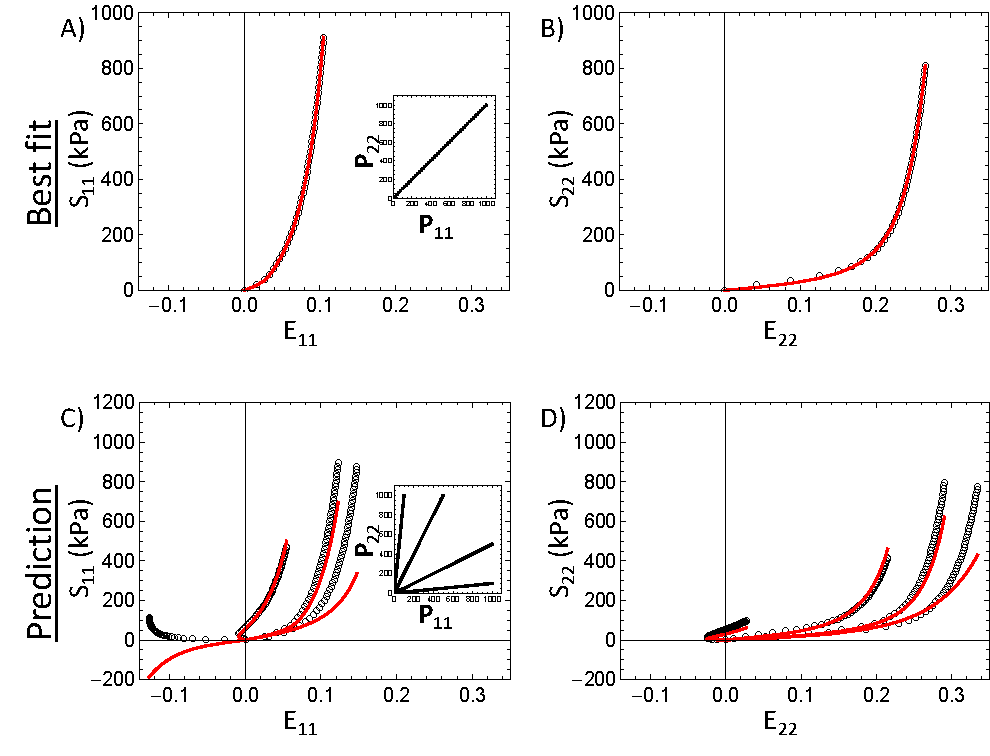
\includegraphics[width=6.5in]{Figures/effequifit}
\caption{$\Psi_{eff}$ fitting to a single equi-biaxial loading path, showing the A) $S_{11}$ and B) $S_{22}$ component. The prediction for the C) $S_{11}$ component and D) $S_{22}$ component of the unfitted loading paths are poor. The inset in C shows the corresponding loading paths.}
\label{fig:effequifit}
\end{figure} 
%-------------------	 end FIGURE 	-------------------%
%%%%%%%%%%%%%%%%%%%%%%%%%%%%%%%%%%%%%%%%%%%%%%%%%%%%%%%%%%%%

	With the addition of other loading paths, even non-optimal, this can significantly improve the predictive capabilities (Fig. \ref{fig:modelspred}A\&B). However, we can clearly see that because the loading paths are not optimal, the $0.1/1$ loading path is not predicted very well (Fig. \ref{fig:modelspred}B). We tested to see if this can be improved through more specific forms of $\Psi_{eff}$ (Eqn. \ref{eqn:finalexponentialmodelformscaled}). For this, we looked at an extension of the generalized Fung model to quadratic terms presented by Sun \textit{et al.} \cite{sun_biaxial_2003} to better fit the response of the glutaraldehyde cross-linked bovine pericardium. The additional terms are only of cubic and quartic powers, $B_{ijkl}E_{ij}^2E_{kl}^2$. In comparison to $\Psi_{eff}$, this is only missing $E_m^3E_n$ and $E_m^3E_n$,
%==========================================================%
%-------------------	begin EQUATION 	-------------------%
\begin{equation}\label{eqn:fullsunmodel}
\begin{aligned}
\Psi	=& c_0 \left(e^{Q} - 1\right) \\
Q		=& A_1 E_{11}^2 + A_2 E_{22}^2 + 2A_3E_{11}E_{22} + A_4 E_{12}^2 + 2A_5E_{12}E_{11}	\\
	&+ 2A_6E_{12}E_{22} + B_1 E_{11}^4 + B_2 E_{22}^4 + 2B_3E_{11}^2E_{22}^2 + B_4 E_{12}^4	\\
    &+ 2B_5E_{12}^2E_{11}^2 + 2B_6E_{12}^2E_{22}^2 
\end{aligned}\tag{Sun et al. \cite{sun_biaxial_2003} Eqn. 4}
\end{equation}
%-------------------	 end EQUATION 	-------------------%
%==========================================================%   
We will call this the extended Fung model. In addition, Sun \textit{et al.} \cite{sun_biaxial_2003} also recommended a more minimalistic form, where only the coupling term $2B_3E_{11}^2E_{22}^2$ is added as , 
%==========================================================%
%-------------------	begin EQUATION 	-------------------%
\begin{equation}\label{eqn:extendedfung}
\begin{aligned}
\Psi	=& c_0 \left(e^{Q} - 1\right) \\
Q		=& A_1 E_{11}^2 + A_2 E_{22}^2 + 2A_3E_{11}E_{22} + A_4 E_{12}^2 + 2A_5E_{12}E_{11}	\\
	&+ 2A_6E_{12}E_{22} + 2B_3E_{11}^2E_{22}^2 + B_4 E_{12}^4.
\end{aligned}
\end{equation}
%-------------------	 end EQUATION 	-------------------%
%==========================================================% 
We shall call this the Sun model. 

	Although the equality of fit are all equally as good \ref{fig:modelsfit}, the extended Fung model (Eqn. \ref{eqn:fullsunmodel}) predicts $S_{22}$ component of the 0.1/1 loading path much better, but predicts the wrong sign for $S_{11}$ for the same loading path, as well as predicting the 1/0.1 loading path worse (Fig. \ref{fig:modelspred}C\&D). The Sun model (Eqn. \ref{eqn:extendedfung}) on the other hand is similar to $\Psi_{eff}$ but worse at predicting $S_{11}$ of the 1/0.1 loading path (Fig. \ref{fig:modelspred}E\&F). It's hard to predict how these constitutive models will behave when the loading paths are not optimal. This is especially true when only a single protocol is used, where predictions for all other protocols can be very poor (Fig. \ref{fig:effequifit}). However, as little as three loading paths are needed to fully reproduce the mechanical response of soft tissue over the entire range of deformations (Fig. \ref{fig:effoptpred}).
%%%%%%%%%%%%%%%%%%%%%%%%%%%%%%%%%%%%%%%%%%%%%%%%%%%%%%%%%%%%
%-------------------	begin FIGURE 	-------------------%
\begin{figure}[!hbtp]
\centering
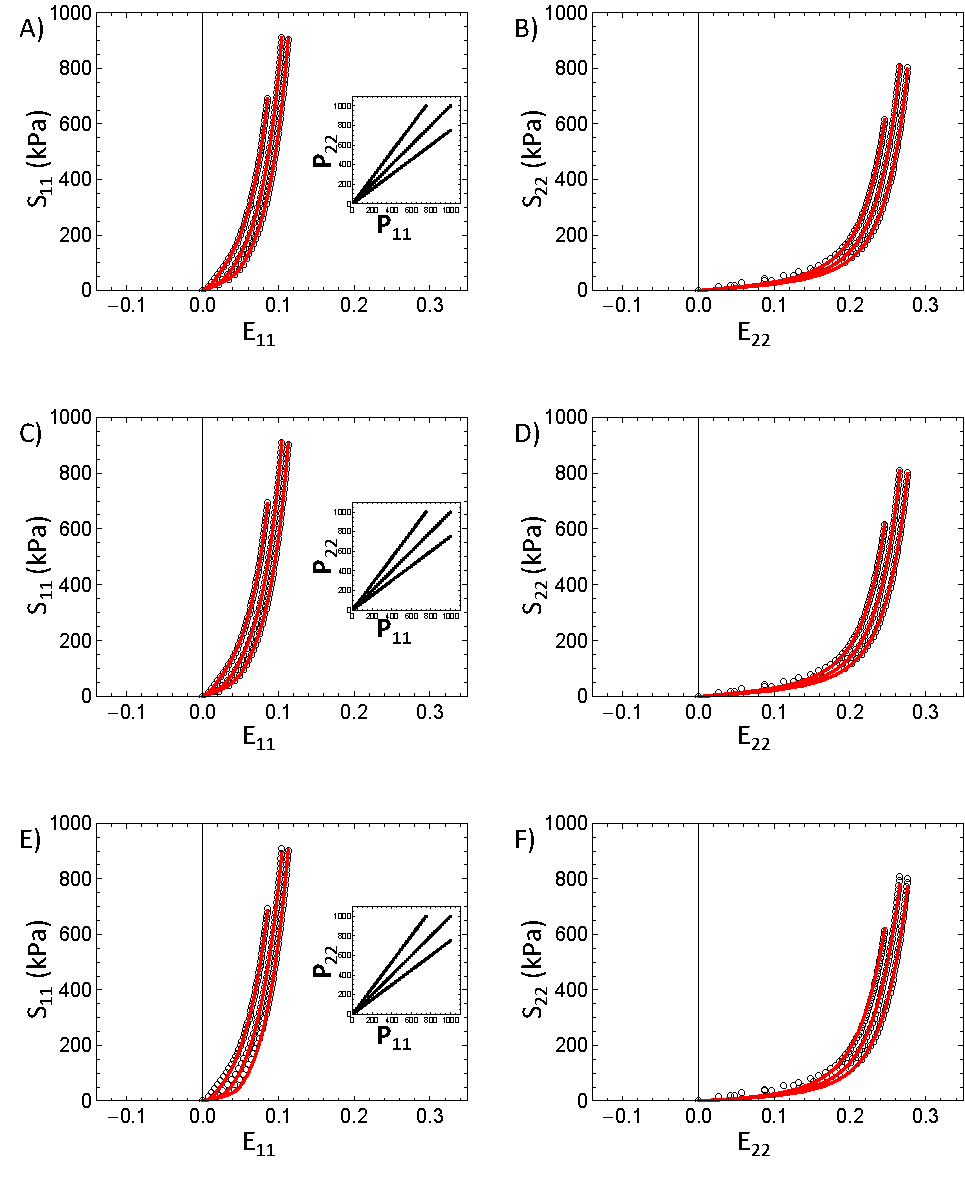
\includegraphics[width=6.5in]{Figures/modelsfit}
\caption{All three models, A\&B) $\Psi_{eff}$ (Eqn. \ref{eqn:finalexponentialmodelformscaled}), C\&D) extended Fung (\ref{eqn:fullsunmodel}), and E\&F) the Sun model (\ref{eqn:extendedfung}), can fit the data equally as well.}
\label{fig:modelsfit}
\end{figure} 
%-------------------	 end FIGURE 	-------------------%
%%%%%%%%%%%%%%%%%%%%%%%%%%%%%%%%%%%%%%%%%%%%%%%%%%%%%%%%%%%%

%%%%%%%%%%%%%%%%%%%%%%%%%%%%%%%%%%%%%%%%%%%%%%%%%%%%%%%%%%%%
%-------------------	begin FIGURE 	-------------------%
\begin{figure}[!hbtp]
\centering
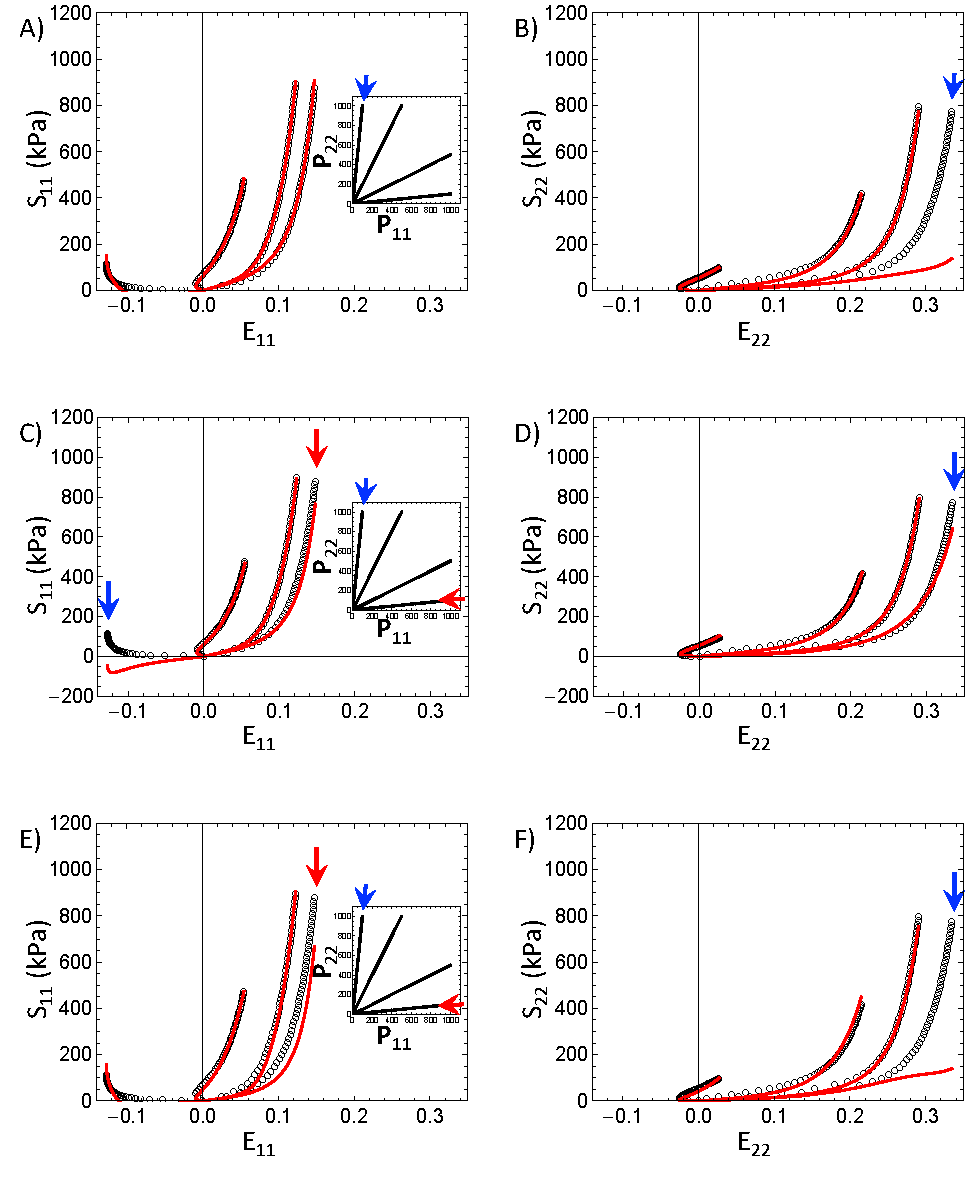
\includegraphics[width=6.5in]{Figures/modelspred}
\caption{Although the quality of fit are all equally as good \ref{fig:modelsfit}), the predictions for the unfitted loading paths are poor because the loading paths that were fit were not optimal. $\Psi_{eff}$ (Eqn. \ref{eqn:finalexponentialmodelformscaled}) predicts A) the $S_{11}$ component well, but B) the $S_{22}$ component of the $0.1/1$ loading path very poorly. The extended Fung (\ref{eqn:fullsunmodel}) predicts C) the $S_{11}$ component of both the $0.1/1$ and $1/0.1$ loading paths poorly, and D) the $S_{22}$ component of the $0.1/1$ loading path poorly. The Sun model (\ref{eqn:extendedfung}) is a slight improvement, only predicting E) the $S_{11}$ component of the $1/0.1$ loading path and F) the $S_{22}$ component of the $0.1/1$ loading path poorly. }
\label{fig:modelspred}
\end{figure} 
%-------------------	 end FIGURE 	-------------------%
%%%%%%%%%%%%%%%%%%%%%%%%%%%%%%%%%%%%%%%%%%%%%%%%%%%%%%%%%%%%




% %%%%%%%%%%%%%%%%%%%%%%%%%%%%%%%%%%%%%%%%%%%%%%%%%%%%%%%%%%%%
% %-------------------	begin FIGURE 	-------------------%
% \begin{figure}[hbtp]
% \centering
% \includegraphics[width=6.5in]{Figures/fungvseff}
% \caption{Comparing the effective constitutive model with the generalized Fung model at fitting the material response of soft tissues, showing the generalized Fung model when fitting to the A) physiological and B) non-physiological loading paths, as well as the effective constitutive model fitting to the C) five most optimal and D) three most optimal loading paths. Alternative types of loading paths were also tested. Including the use of p- and l-protocols in the post-pre-strain (p-p-E) range defined in Fung \textit{et al.} \cite{fung_pseudoelasticity_1979}. In this case, we shown the results for using D) one pair and F) three pairs of such protocols. Column 1-3 shows the quality of fit for each case, and column 4 shows the ability of the constitutive models to predict the remaining loading paths.}
% \label{fig:fungvseff}
% \end{figure} 
% %-------------------	 end FIGURE 	-------------------%
% %%%%%%%%%%%%%%%%%%%%%%%%%%%%%%%%%%%%%%%%%%%%%%%%%%%%%%%%%%%%


    
    

% %%%%%%%%%%%%%%%%%%%%%%%%%%%%%%%%%%%%%%%%%%%%%%%%%%%%%%%%%%%%
% %-------------------	begin FIGURE 	-------------------%   
% \begin{figure}
% \centering
% \includegraphics[width=6.5in]{Figures/nonoptimalpaths}
% \caption{Comparing parameter estimation results when fitting to non-optimal loading paths, using A) $\Psi_{eff}$ (Eqn. \ref{eqn:finalexponentialmodelformscaled}) and two other extensions to the generalized Fung models from Sun \textit{et al.} \cite{sun_biaxial_2003}, B) equation 4, which is an extension to the generalized Fung model by adding the quartic terms of $E_{11}^4$, $E_{22}^4$, $E_{12}^4$, $E_{11}^2 E_{22}^2$, $E_{11}^2 E_{12}^2$, and $E_{22}^2 E_{12}^2$ and C) equation 5 of said work, which is an extension to the generalized Fung model by adding the term $E_{11}^2 E_{22}^2$ only. D) $\Psi_{eff}$ was also fitted to only the equi-biaxial tension loading path and check for it's abilities to predict the remaining responses.}
% \label{fig:nonoptimalpaths}
% \end{figure} 
% %-------------------	 end FIGURE 	-------------------%
% %%%%%%%%%%%%%%%%%%%%%%%%%%%%%%%%%%%%%%%%%%%%%%%%%%%%%%%%%%%%











